% Part: sets-functions-relations
% Chapter: infinite
% Section: hilberts-hotel
%
\documentclass[../../../include/open-logic-section]{subfiles}

\begin{document}

\olfileid[tr]{sfr}{infinite}{hilbert}
\olsection{Hilbert'in Oteli}

Doğal sayılar kümesinin sonsuz olduğu açıktır. Dolayısıyla doğal sayıları
hazırdan \emph{kullanmak} istemiyorsak ilk adımımız, sonsuz bir kümeyi doğal
sayıların kendilerinden söz etmeyi gerektirmeyen terimlerle tanımlamak
olmalıdır. Hilbert'in 1924 tarihli bir dersinde sunduğu güzel yaklaşım
şöyledir. Bizden şunu hayal etmemizi ister:
\begin{quote}
[\ldots] sonlu sayıda odası olan bir otel. Bu odaların her birinde tam bir
konuk kalıyor olsun. Konuklar şimdi odalarını bir biçimde değiştirse, [ama]
her odada yine en çok bir kişi kalacak biçimde değiştirse, hiçbir oda
boşalmaz ve otel sahibi bu yolla yeni gelen bir konuk için yeni bir yer
açamaz [\ldots
\textparagraph \ldots]

Şimdi otelde her biri tam bir konuk tarafından kullanılan, numaralanmış
sonsuz sayıda oda bulunduğunu kabul edelim: $1$, $2$, $3$, $4$, $5$, \dots.
Yeni bir konuk gelir gelmez otel sahibinin eski konukların her birini yalnızca
numarası bir büyük olan odaya taşıması gerekir; böylece oda~$1$ yeni gelen
konuk için boşalır.
	\begin{center}
		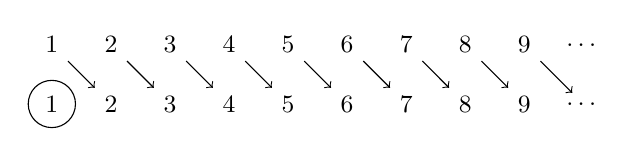
\begin{tikzpicture}[scale = .75]
		\foreach \x in {1, 2, 3, 4, 5, 6, 7, 8, 9}
		{
			\node (\x a) at (\x, 1) {\small{\x}};
			\node (\x b) at (\x, 2) {\small{\x}};
		}
		\node (dotsa) at (10, 1) {\small{\ldots}};
		\node (dotsb) at (10, 2) {\small{\ldots}};
		\draw[->] (1b)--(2a);
		\draw[->] (2b)--(3a);
		\draw[->] (3b)--(4a);
		\draw[->] (4b)--(5a);
		\draw[->] (5b)--(6a);
		\draw[->] (6b)--(7a);
		\draw[->] (7b)--(8a);
		\draw[->] (8b)--(9a);
		\draw[->] (9b)--(dotsa);
		\draw (1,1) circle (.4);
		\end{tikzpicture}
	\end{center}
	(\citealt[730]{EwaldSieg2013}'te yayımlanmıştır; çeviri bize ait)
\end{quote}
Kilit nokta, Hilbert'in Oteli'nin sonsuz sayıda odası olmasıdır; onun
açıklamasını, bunu söylemenin ne anlama geldiğini tanımlamak için
kullanabiliriz. Nitekim Dedekind'in yaklaşımı da buydu (burada elbette
büyük bir tarih yanılgısıyla sunuyoruz; Dedekind'in tanımı
\citeyear{Dedekind1888} tarihlidir):

\begin{defn}\ollabel{defn:DedekindInfinite}
Bir $A$ kümesi, ancak ve ancak $A$'dan $A$'nın bir öz alt kümesine !!a{injection}
varsa \emph{Dedekind anlamında sonsuzdur}. Başka bir deyişle, bir $o\in A$
ve $o\notin\ran{f}$ olacak biçimde bir !!a{injection}
$f\colon A\to A$ vardır.
\end{defn}

\end{document}
